% ============================================================
% Chapter 4: Design
% ============================================================
\chapter{Design}
\label{ch:design}

The experimental contributions of Chapters~\ref{ch:detection}, \ref{ch:classification}, and~\ref{ch:deployment} rest on a common methodological foundation. Every downstream experimental claim depends on the design decisions established here, from how the system is formally modeled and data is partitioned, to which features are constructed and how performance is evaluated. This chapter establishes that foundation: the formal monitoring system model (\S\ref{sec:monitoring-system}), the experimental datasets (\S\ref{sec:datasets}), the data pipeline and exploratory analysis (\S\S\ref{sec:pipeline-architecture}--\ref{sec:eda}), the splitting, preprocessing, and feature engineering protocols (\S\S\ref{sec:splitting}--\ref{sec:feature-engineering}), the evaluation methodology (\S\ref{sec:evaluation-methodology}), and the edge deployment context (\S\ref{sec:deployment-architecture}).

% ────────────────────────────────────────────────────────────
\section{Proposed Monitoring System}
\label{sec:monitoring-system}
% ────────────────────────────────────────────────────────────

The system proposed in this work targets photovoltaic installations operating under field conditions and provides 2 complementary diagnostic capabilities: continuous detection of deviations from the expected operating envelope, and, when such a deviation is confirmed, identification of the specific fault type responsible. This section formalizes the physical system, the observable measurement space, the fault model, and the mathematical formulation of the 2 diagnostic tasks.

\subsection{Physical System and Measurement Model}

Consider a photovoltaic installation comprising a set $\mathcal{S}$ of strings, each composed of $N$ photovoltaic modules $\{\mathrm{PV}_1, \mathrm{PV}_2, \ldots, \mathrm{PV}_N\}$ connected in series. When subject to an irradiance $G$~(W/m$^2$) and ambient temperature $T$~($^\circ$C), an arbitrary string $s \in \mathcal{S}$ generates a DC voltage $V_{\mathrm{dc},s}$ and a DC current $I_{\mathrm{dc},s}$, from which its output power follows as $P_{\mathrm{dc},s} = V_{\mathrm{dc},s} \cdot I_{\mathrm{dc},s}$. Both quantities are functions of $G$ and $T$: the output current scales approximately linearly with irradiance, while the open-circuit voltage decreases linearly with temperature above the standard test condition reference of 25\,$^\circ$C, at a rate specified by the module temperature coefficient. An inverter aggregates the DC output of all strings in $\mathcal{S}$ and converts the combined power into an alternating-current waveform characterized by voltage $V_{\mathrm{ac}}$ and current $I_{\mathrm{ac}}$; the resulting power $P_{\mathrm{ac}} = V_{\mathrm{ac}} \cdot I_{\mathrm{ac}}$ is injected into the utility grid.

A data acquisition system samples the complete set of electrical and meteorological quantities, $\{V_{\mathrm{dc},s},\, I_{\mathrm{dc},s}\}_{s \in \mathcal{S}},\; V_{\mathrm{ac}},\; I_{\mathrm{ac}},\; G,\; T$, at a fixed sampling frequency, producing a multivariate time series $\mathbf{x}(t) \in \mathbb{R}^d$ at regular discrete intervals. Under normal operating conditions, the measured quantities follow an expected relationship governed by standard photovoltaic physics. Any departure from this expected relationship that cannot be explained by ordinary variations in $G$ or $T$ constitutes the observable evidence of a fault condition.

\subsection{Fault Model}

A fault condition is any persistent deviation of the measured electrical quantities from their expected values under the observed irradiance and temperature. Such deviations arise from changes in the physical integrity of the installation: resistive degradation of contacts, interruption of current paths, reduction in effective module area, or modification of the string electrical characteristics. The monitoring system treats each such condition as a discrete class to be identified. The specific fault types present in a given deployment are determined by the operational context and are introduced through the experimental datasets described in Section~\ref{sec:datasets}.

\subsection{Diagnostic Cascade}

The monitoring system responds to fault conditions through a 2-stage diagnostic cascade illustrated in Figure~\ref{fig:monitoring-system}. The first stage, \emph{fault detection}, processes a window $\mathbf{X}(t) = [\mathbf{x}(t-w+1), \ldots, \mathbf{x}(t)] \in \mathbb{R}^{w \times d}$ of the $w$ most recent measurement vectors and returns a binary decision:
\[
    d(t) \;=\; \begin{cases} 1 & \text{if a fault condition is detected,} \\ 0 & \text{otherwise.} \end{cases}
\]
This stage is formulated as a semi-supervised anomaly detection problem. The detector learns a statistical characterization of normal operation from historical normal-class data and flags any window whose anomaly score exceeds a calibrated threshold, without requiring labeled fault examples at training time.

The second stage, \emph{fault classification}, is triggered only when $d(t) = 1$ and assigns the anomalous window to one of $K$ fault classes, producing a label $\hat{y}(t) \in \{1, \ldots, K\}$. The classification result, together with its confidence score and timestamp, is presented to the plant operator through the monitoring interface described in Chapter~\ref{ch:deployment}. The 2-stage design reflects the operational reality that a plant operator needs first to be informed that something has changed, and only then to be told what has changed; the 2 questions are answered by qualitatively different statistical procedures with different assumptions about the availability of labeled training data.

\begin{figure}[H]
\centering

\includegraphics[width=\textwidth]{monitoring system formulation}
\caption{High-level architecture of the proposed 2-stage fault monitoring system.}
\label{fig:monitoring-system}
\end{figure}

% ────────────────────────────────────────────────────────────
\section{Experimental Datasets}
\label{sec:datasets}
% ────────────────────────────────────────────────────────────

The experiments in this work are conducted on 2 independent field datasets. The Costa dataset \citep{costa2020sensors} is the primary experimental resource: it covers 4 electrically distinct fault types induced on real hardware under controlled conditions, making it the natural candidate for multi-class fault classification and the main evaluation surface for anomaly detection. The La Réunion dataset \citep{graillet2023dib} serves as a generalization benchmark: recorded on a separate continent under a tropical climate with a different hardware configuration and a shading-only fault taxonomy, it allows the pipeline architecture to be validated across heterogeneous field conditions through an independent execution on a structurally distinct site. The two sites differ in geographic location, climate, installed capacity, module technology, acquisition infrastructure, and fault induction protocol.

\paragraph{Costa.}
The Costa installation is a 5~kW photovoltaic system located in Curitiba, Paraná, Brazil (25.4°S, 49.3°W) \citep{costa2020sensors}. The plant consists of 2 strings of 8 Canadian Solar CS6U-330P poly-crystalline modules each ($N = 16$ modules, 330~W rated power per module). A National Instruments CompactRIO controller equipped with signal acquisition modules and programmed in LabVIEW acquires per-string DC voltage $V_{\mathrm{dc},s}$ and DC current $I_{\mathrm{dc},s}$ for both strings, together with the AC voltage $V_{\mathrm{ac}}$ and AC current $I_{\mathrm{ac}}$ at the inverter output, all at a sampling frequency of 1~Hz. A co-located weather station records global irradiance $G$ [W~m$^{-2}$] via an EKO MS-40 class B pyranometer and panel back-surface temperature $T$ [°C] via PT100 contact sensors, also at 1~Hz, with ambient temperature, relative humidity, and wind speed logged as secondary meteorological variables.

The dataset covers 5 operating conditions: normal operation (label~0), short circuit between adjacent modules (label~1), high-resistance degradation contact (label~2), open circuit of a string (label~3), and partial shadowing (label~4). The fault type is recorded as a discrete label column. The dataset covers 16~days of continuous recording at 1~Hz, totalling 1\,373\,798 samples \citep{costa2020sensors}. Table~\ref{tab:costa-vars} lists the ingested columns.

\begin{table}[H]
\centering
\caption{Costa dataset: recorded variables and fault label encoding.}
\label{tab:costa-vars}
\begin{tabular}{l p{7.5cm} c}
\toprule
\textbf{Column} & \textbf{Description} & \textbf{Unit} \\
\midrule
\texttt{vdc1} & String 1 DC voltage & V \\
\texttt{idc1} & String 1 DC current & A \\
\texttt{pdc1} & String 1 DC power ($= \mathtt{vdc1} \times \mathtt{idc1}$) & W \\
\texttt{vdc2} & String 2 DC voltage & V \\
\texttt{idc2} & String 2 DC current & A \\
\texttt{pdc2} & String 2 DC power ($= \mathtt{vdc2} \times \mathtt{idc2}$) & W \\
\texttt{pdc}  & Total DC power ($= \mathtt{pdc1} + \mathtt{pdc2}$) & W \\
\texttt{irr}  & Global irradiance & W~m$^{-2}$ \\
\texttt{pvt}  & PV module back-surface temperature & $^\circ$C \\
\texttt{label} & Fault class: 0 Normal; 1 ShortCircuit; 2 Degradation; 3 OpenCircuit; 4 Shadowing & -- \\
\bottomrule
\end{tabular}
\end{table}

\newpage
\paragraph{La Réunion.}
The La Réunion installation is a 4~kW rooftop photovoltaic system located on the campus of the University of La Réunion, Saint-Denis, La Réunion Island, Indian Ocean (20.9°S, 55.5°E) \citep{graillet2023dib}. The plant comprises 2 inverter lines, each consisting of 12 polycrystalline modules (Total Energie) arranged as 2 parallel series of 6 panels, mounted at a tilt angle of 26°. The inverter line on which faults are induced (line~1) operates alongside a second line (line~2) kept in normal conditions throughout the experiments, providing a contemporaneous control reference under identical irradiance. Electrical production data (AC power $P_g$, AC voltage $V_a$, AC current $I_a$, grid current $I_g$, grid voltage $V_g$, and grid frequency $F_g$) are acquired per inverter line through an Energrid datalogger at 0.2~Hz (one sample every 5~seconds). Meteorological quantities (global and diffuse tilted irradiance GTI and DTI [W~m$^{-2}$], and module back-surface temperature $T_{\mathrm{PV}}$ [°C]) are recorded at 1~Hz via a Campbell Scientific CR1000X datalogger equipped with a Delta-T Devices SPN1 pyranometer and type-T and type-K thermocouples. Data are transmitted over TCP/IP and stored in an InfluxDB time-series database; the dataset spans October~2021 to April~2023, totalling 2\,988\,814 samples, and is publicly available on Zenodo \citep{graillet2023dib}.

Fault conditions correspond exclusively to shading variants, each induced by applying an opaque mask to the relevant modules: uniform shading of the entire line (label~1), constant partial shading of 1 to 3 complete modules (labels~2.1--2.3), constant partial shading of fractions of a single module (labels~3.1--3.2), and static intermittent partial shading produced by a fixed shadow-casting object (label~4). The fault type is recorded as a numeric variable directly in the database at the time of induction. Because all fault conditions involve some form of irradiance reduction rather than an electrical integrity change, the La Réunion fault taxonomy is structurally narrower than Costa's. This difference motivates its role as a pipeline generalization benchmark rather than as a primary classification dataset. Table~\ref{tab:reunion-vars} lists the ingested columns.

\begin{table}[H]
\centering
\caption{La Réunion dataset: recorded variables and fault label encoding.}
\label{tab:reunion-vars}
\begin{tabular}{l p{7.5cm} c}
\toprule
\textbf{Column} & \textbf{Description} & \textbf{Unit} \\
\midrule
\texttt{Ia}    & Inverter AC current & A \\
\texttt{Ig}    & Grid AC current & A \\
\texttt{Va}    & Inverter AC voltage & V \\
\texttt{Vg}    & Grid AC voltage & V \\
\texttt{Pg}    & Grid AC power & W \\
\texttt{Eg}    & Energy injected to grid & kWh \\
\texttt{Fg}    & Grid frequency & Hz \\
\texttt{GTI}   & Global tilted irradiance & W~m$^{-2}$ \\
\texttt{DTI}   & Diffuse tilted irradiance & W~m$^{-2}$ \\
\texttt{TA}    & Ambient air temperature & $^\circ$C \\
\texttt{TPV}   & PV module back-surface temperature & $^\circ$C \\
\texttt{label} & Fault class: 0 Normal; 1 Uniform shading; 2.1--2.3 Constant partial shading (1--3 modules); 3.1--3.2 Partial module fraction; 4 Intermittent shading & -- \\
\bottomrule
\end{tabular}
\end{table}

% ────────────────────────────────────────────────────────────
\section{Pipeline Architecture}
\label{sec:pipeline-architecture}
% ────────────────────────────────────────────────────────────

The data pipeline that transforms raw field recordings into the inference-ready representations consumed by every modeling experiment is organized as 5 sequential stages: ingestion, splitting, preprocessing, feature engineering, and model training. This staged organization is a deliberate architectural choice rather than an implementation convenience. A monolithic transformation script would make it impossible to enforce leakage-prevention invariants at a well-defined boundary, to rebuild expensive downstream stages independently when upstream logic changes, or to apply the same pipeline to a new field dataset without touching the transformation code. The staged structure addresses all 3 requirements simultaneously and is the structural foundation of the portability claim: the same pipeline code, parameterized by a site-specific configuration file, produces independent artifact trees for each field dataset with no shared internal state.

The pipeline is managed through a declarative dependency graph whose manifest records the code, configuration, and data inputs of each stage explicitly. Any modification to an upstream stage automatically invalidates its downstream artifacts, forcing their regeneration rather than silent reuse of stale results. All intermediate artifacts are namespaced by dataset and task, so that adding a new field site requires only a configuration change. Figure~\ref{fig:pipeline} illustrates the complete pipeline and the role of each stage.

\begin{itemize}
    \item \textbf{Ingestion} converts raw sensor logs from a given field site into a unified operational table: acquisition streams recorded by heterogeneous systems at different sampling frequencies are joined and aligned, night-time observations below 100~W/m$^2$ irradiance are discarded, and the fault condition is assigned to a single shared label column. This conversion is the only stage that carries site-specific format knowledge; every downstream stage receives an identical schema and is fully insulated from the acquisition details of the source system.
    \item \textbf{Splitting} partitions the consolidated table into training, validation, and test sets according to the temporal grouping protocol described in Section~\ref{sec:splitting}. No sample-level transformation is performed at this stage; splitting is the gate at which evaluation integrity is established, and it must precede all subsequent stages that estimate statistics from the data.
    \item \textbf{Preprocessing} cleans the normal-class rows of the training partition through outlier removal (fault-labeled rows are exempt, as extreme values in those rows are expected fault signatures) and, for sites where the exploratory analysis identifies sustained temporal gaps in the field recording, tiered missing-value imputation (Section~\ref{sec:preprocessing}), then estimates all cleaning statistics exclusively from that partition and applies them as fixed constants to validation and test.    \item \textbf{Feature engineering} transforms cleaned measurements into the representations consumed by the downstream models: named profiles specify which feature families are constructed, and a train-only selection stack eliminates redundant and low-relevance candidates before the final feature tables are written to disk. The profile system makes this stage a controlled ablation instrument, isolating the contribution of each feature family across experiments.
    \item \textbf{Model training} fits each candidate model on the feature-engineered partitions, restricts hyperparameter optimisation strictly to the training and validation partitions, and computes final metrics on the test partition exactly once after the winning configuration has been selected. All configurations, trained artifacts, and evaluation results are logged to a remote experiment tracking server, making every reported figure traceable to a specific run.
\end{itemize}

\begin{figure}[H]
\centering
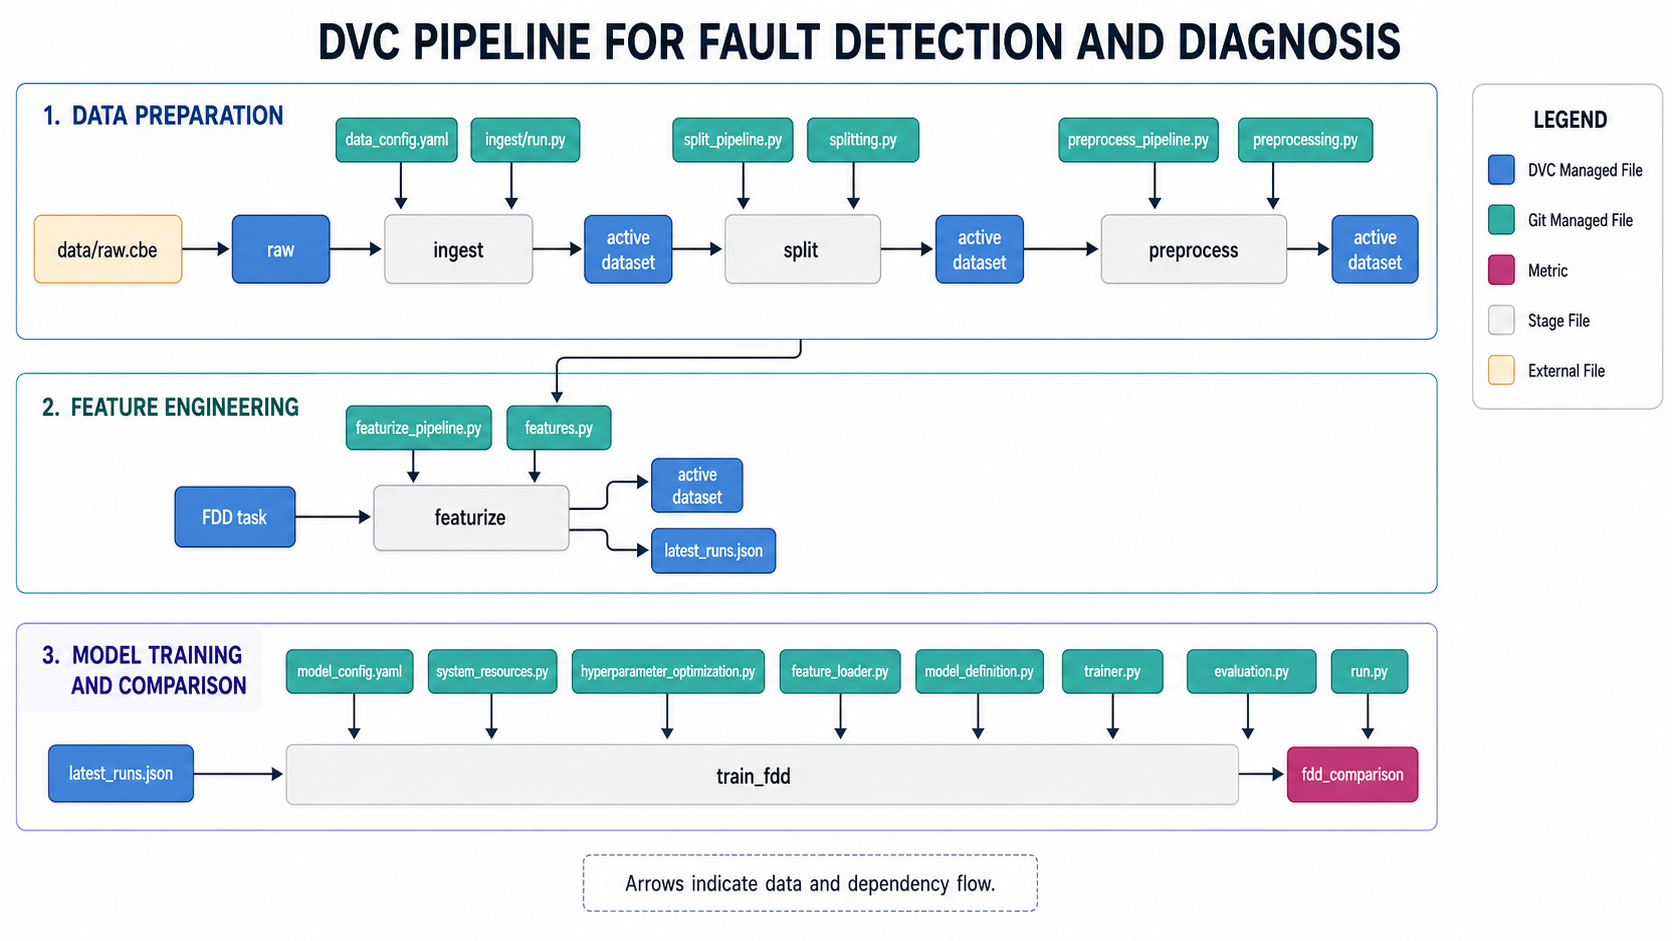
\includegraphics[width=\textwidth]{figures/dvc pipeline.png}
\caption{Five-stage data pipeline from raw field recordings to model training and edge deployment.}
\label{fig:pipeline}
\end{figure}

% ────────────────────────────────────────────────────────────
\section{Exploratory Data Analysis}
\label{sec:eda}
% ────────────────────────────────────────────────────────────

Before any model is trained, a systematic exploratory analysis of the raw and cleaned field measurements was conducted to identify structural properties of the data that would inform both the preprocessing design and the feature engineering choices. Four findings from this analysis had direct and traceable consequences for the system design.

The first finding concerns algebraic redundancy among the measured channels. The per-string power columns are deterministic functions of the corresponding voltage and current columns by the identity $P_{\mathrm{dc},s} = V_{\mathrm{dc},s} \cdot I_{\mathrm{dc},s}$, and the total DC power is the algebraic sum of the per-string powers. Including both the primary and derived channels in the candidate feature pool creates exact linear dependencies that inflate the nominal feature dimensionality without providing independent information. This observation motivates the first stage of the feature selection stack described in Section~\ref{sec:feature-engineering}, which detects and removes deterministic aliases before any model is fitted.

The second finding concerns the dominant linear relationship between irradiance and electrical output. Under normal operating conditions, the per-string DC current and total output power exhibit Pearson correlation coefficients with the incident irradiance $G$ that exceed 0.90 across all examined field recordings. This strong linear dependence means that the raw electrical channels carry a large irradiance-driven component that would dominate any model trained on untransformed measurements. Normalizing the power and current channels by irradiance isolates the irradiance-residual, which is the quantity most sensitive to fault-related deviations because it reflects changes in the system's conversion efficiency rather than changes in the solar resource. This observation is the direct motivation for the irradiance-normalized feature family at the core of the \texttt{plus\_physics} profile described in Section~\ref{sec:feature-engineering}.

The third finding concerns class imbalance in both field datasets. Normal-operation samples constitute the overwhelming majority of the recorded observations, while fault-labeled intervals account for a small minority of the total recording duration. This distributional asymmetry has 2 direct consequences for the experimental design. First, it motivates the choice of the area under the precision-recall curve as the primary metric for the anomaly detection task, because the receiver-operating-characteristic curve area is structurally insensitive to severe class imbalance and would assign a near-perfect score to a trivial all-negative classifier. Second, it motivates the semi-supervised training protocol for Task~A, in which the detector learns exclusively from normal-class data and is evaluated on mixed partitions, reflecting the realistic scenario in which labeled fault material is scarce or unavailable at training time.

The fourth finding is specific to multi-string installations. The individual per-string voltage and current channels provide differential information not visible in plant-aggregated quantities: a localized fault on one string produces a detectable asymmetry between per-string measurements that is diluted or entirely invisible in the total output power. This observation motivates the per-string imbalance descriptors included in the \texttt{plus\_physics} profile, which exploit the natural redundancy of the multi-string architecture to expose localized fault signatures.

% ────────────────────────────────────────────────────────────
\section{Splitting Protocol}
\label{sec:splitting}
% ────────────────────────────────────────────────────────────

Splitting is the stage at which the conditions for honest evaluation are either established or fatally compromised. The protocol adopted in this work rests on 3 principles, each enforced by a concrete implementation safeguard.

\textbf{Principle 1: Grouped atomic units.} A photovoltaic time series sampled at 1~Hz contains dense local autocorrelation: consecutive samples carry nearly identical information, and assigning some of them to the training partition and others to the test partition does not produce an independent evaluation surface. The atomic unit for partitioning is a contiguous run of temporally adjacent measurements, bounded by a temporal gap exceeding 300~seconds or by a fault label transition. No atomic unit is ever fragmented across partitions. This design eliminates the most direct form of row-level contamination and ensures that the evaluation reflects the model's ability to generalize to genuinely unseen operating episodes rather than to held-out samples from episodes already observed in training.

\textbf{Principle 2: Temporal ordering with embargoed boundaries.} Partitions are assigned in strict chronological order: the maximum timestamp of the training partition precedes the minimum timestamp of the validation partition, which in turn precedes the minimum timestamp of the test partition. A 1260-second (21-minute) embargo is enforced between adjacent partition boundaries, so that no feature computed at evaluation time can depend on samples from an earlier partition even through long rolling windows. The embargo duration is set as a conservative multiple of the longest rolling window used in the feature engineering stage.

\textbf{Principle 3: Post-split windowing.} Sliding windows are constructed strictly within the boundaries of each partition, never across them. Window construction before splitting would allow overlapping windows to share samples from multiple partitions, creating a leakage channel that cannot be repaired retroactively. By deferring windowing to after the partition boundaries have been fixed, no 2 windows in different partitions ever share an underlying sample.

The partition ratios are 70 / 15 / 15 for training, validation, and test respectively. For Task~A (anomaly detection), the training partition contains only normal-class atomic units, reflecting the semi-supervised assumption that labeled fault patterns are not available at training time; validation and test partitions contain the full label range and represent the realistic deployment scenario. For Task~B (fault classification), atomic units are distributed across all 3 partitions with temporal-stratified assignment per fault class, so that each class has representation in all partitions while temporal ordering is preserved within each class.

% ────────────────────────────────────────────────────────────
\section{Preprocessing}
\label{sec:preprocessing}
% ────────────────────────────────────────────────────────────

Preprocessing is conceived as a minimal cleaning layer that intervenes between split assignment and feature engineering. The guiding principle is that the model must learn to detect deviations from the expected operating behavior, and the preprocessing stage must preserve this signal while staying as lean as the underlying data quality allows. The preprocessing intensity is therefore calibrated per dataset rather than imposed as a uniform recipe.

For field recordings where the daytime-filtered measurement sequence contains no systematic missing-value problem, the active preprocessing layer consists of a single operation: scope-limited outlier removal applied to the primary measured channels. The interquartile range of each primary electrical channel is computed exclusively on the normal-class rows of the training partition, and any normal-class training row whose value falls outside a bound of $3 \times \mathrm{IQR}$ is dropped. Fault-class rows are never subjected to outlier removal, because the extreme values present in those rows are precisely the signatures that the detection and classification systems are expected to learn. The multiplier of 3 (rather than the more aggressive value of 1.5) is chosen to target only values attributable to sensor malfunction or acquisition errors rather than to legitimate operational variability. Derived power channels are recomputed deterministically from the cleaned primary channels after outlier removal, which preserves the algebraic identity $P_{\mathrm{dc},s} = V_{\mathrm{dc},s} \cdot I_{\mathrm{dc},s}$ and prevents spurious mismatches between primary and derived quantities.

For field recordings that expose longer temporal gaps in the raw sequence, a tiered imputation policy supplements the outlier removal step. Gaps shorter than 60~seconds are filled by forward propagation of the last observed value, on the assumption that such gaps reflect transient sensor interruptions during which the underlying physical state is unlikely to have changed materially. Gaps between 60 and 300~seconds are filled by linear interpolation between the bracketing observations, under the assumption that the physical variables vary smoothly over this time scale in the absence of a fault event. Gaps exceeding 300~seconds are dropped regardless of their origin, because no defensible interpolation strategy applies to windows in which the operational state of the plant may have changed substantially. A non-negotiable rule overrides these thresholds whenever a gap overlaps with a fault-labeled period: any such gap is dropped without imputation, because interpolating values on a fault-labeled segment would fabricate fault signatures that the detection system is expected to identify rather than assume.

A general invariant is enforced across all preprocessing decisions. Any statistic estimated from the data, including outlier bounds, imputation parameters, and normalization factors, is computed exclusively from the training partition and applied as a constant to the validation and test partitions. This discipline preserves the independence of the evaluation surface and prevents any form of look-ahead leakage through preprocessing.

% ────────────────────────────────────────────────────────────
\section{Feature Engineering and Profile Ablation}
\label{sec:feature-engineering}
% ────────────────────────────────────────────────────────────

The feature engineering stage transforms cleaned operational measurements into the representations consumed by the downstream models. Two design principles govern its implementation. The first is that features are organized into named profiles, each corresponding to a coherent ablation level that strictly extends its predecessor, enabling a principled comparison of feature representations by contrasting adjacent profile levels. The second is that all selection statistics are estimated exclusively from the training partition, in keeping with the leakage-prevention discipline established in Section~\ref{sec:splitting}.

\subsection{Physics-Informed Features}

The starting point of the profile ladder is a compact set of physics-informed features motivated directly by the exploratory observations of Section~\ref{sec:eda}. These features encode domain knowledge about photovoltaic operation that a purely data-driven model would otherwise have to rediscover from raw observations, and they are constructed to remain numerically stable across the full operating range of the installation.

The first family normalizes power and current channels by the incident irradiance. Under healthy operation, the ratios $P_{\mathrm{dc},s} / G$ and $I_{\mathrm{dc},s} / G$ are approximately constant because irradiance is the dominant driver of both quantities. Normalization collapses the large diurnal amplitude swing present in the raw channels and exposes the fault-related residual that carries the diagnostic signal. The denominator is floored at 1~W/m$^2$ to prevent numerical instability at dawn and dusk.

The second family is the per-string imbalance descriptors. For multi-string installations where each string is individually instrumented, the normalized difference between per-string currents, voltages, and powers provides a sensitive indicator of localized faults that do not manifest in plant-aggregated quantities. Three imbalance features (power imbalance, current imbalance, and voltage imbalance) are computed as normalized pairwise differences and exploit the natural redundancy of the multi-string architecture.

The third family is the temperature-corrected power. The maximum power point of crystalline silicon modules decreases approximately linearly with temperature above the 25\,$^\circ$C standard test condition reference, at a rate given by the module-specific temperature coefficient $\gamma_{P_{\mathrm{max}}}$. The temperature-corrected power divides the observed output by the expected thermal loss factor, and its further normalization by irradiance produces a feature that isolates the fault-related power deviation from the component attributable to ordinary thermal behavior.

The fourth family comprises the first-order temporal derivatives of the primary channels ($\mathrm{d}P/\mathrm{d}t$, $\mathrm{d}V/\mathrm{d}t$, and $\mathrm{d}I/\mathrm{d}t$), computed as discrete differences between consecutive cleaned samples. Rapid transients in current or voltage are characteristic of certain fault types, particularly short circuits and open circuits, and these derivative features expose such transients more clearly than the raw values when the absolute magnitude of the signal is large.

Together, the 4 families yield approximately 17 engineered features after the selection stack described below has pruned the candidate pool. This feature set defines the profile \texttt{plus\_physics}, which serves as the principal representation for the headline experiments in Chapters~\ref{ch:detection} and~\ref{ch:classification}.

\subsection{Profile Ladder}

The named profiles form an additive ablation ladder in which each rung strictly extends the one below it. The 4 profiles evaluated in this thesis are as follows:

\begin{itemize}
    \item \texttt{baseline\_raw}: the cleaned sensor columns produced by preprocessing, with no engineered features. This profile provides the reference level against which the contribution of feature engineering is measured. The hygiene pruning step described below is the only selection applied.
    \item \texttt{plus\_physics}: extends \texttt{baseline\_raw} by adding the 4 physics-informed feature families described above and applying the full hygiene-plus-mRMR selection stack. This is the primary profile used for the headline results in the contribution chapters.
    \item \texttt{plus\_temporal}: extends \texttt{plus\_physics} by adding cyclic encoding of the time of day, representing the hour and minute as sine and cosine projections so that the model receives a continuous, smooth representation of diurnal position without a discontinuity at midnight.
    \item \texttt{plus\_rolling}: extends \texttt{plus\_temporal} by adding causal rolling statistics (rolling mean and rolling standard deviation) over short causal windows, providing the model with a compact summary of recent history that remains strictly within the training partition boundaries.
\end{itemize}

\subsection{Selection Stack}

The candidate feature pool is pruned by a 2-stage train-only selector stack before the final feature set is written to disk. The first stage is hygiene pruning: near-constant columns whose variance falls below a numerical threshold are removed, exact duplicate columns are collapsed, and deterministic algebraic aliases (such as the identity $P_{\mathrm{dc}} = P_{\mathrm{dc},1} + P_{\mathrm{dc},2}$ identified during exploratory analysis) are detected and reduced to a single representative. This stage requires no label information and therefore introduces no leakage risk.

The second stage applies minimum-redundancy maximum-relevance (mRMR) feature selection under the mutual information difference (MID) criterion \citep{peng2005mrmr}, with a target retained pool of 64 features after hygiene. The relevance term scores each candidate by its mutual information with the task label; the redundancy term penalizes mutual information against already-retained features; the greedy selection proceeds until the target size is reached or the pool is exhausted. All mutual information estimates are computed from the training partition only. For large training partitions, estimation is performed on a stratified, group-aware subset of up to 30\,000 rows, which preserves the statistical structure of the label distribution and the temporal grouping while keeping the selection step tractable within the project's computational budget.

% ────────────────────────────────────────────────────────────
\section{Evaluation Methodology}
\label{sec:evaluation-methodology}
% ────────────────────────────────────────────────────────────

Honest evaluation is the discipline that connects the data pipeline to the scientific claims of this thesis. The methodology combines a deliberate choice of headline metrics, a non-negotiable leakage validation suite, a controlled hyperparameter optimization protocol, and a statistical significance procedure that distinguishes meaningful from cosmetic improvements.

\subsection{Headline Metrics}

For Task~A the primary metric is the area under the precision-recall curve (PR-AUC). On field datasets where normal-operation samples constitute the overwhelming majority of the recorded sequence, the area under the receiver-operating-characteristic curve (ROC-AUC) is structurally misleading: a classifier that assigns the negative label to every sample achieves near-perfect accuracy and an ROC-AUC approaching 1.0, neither of which conveys operational meaning. The precision-recall curve measures directly the trade-off between the fraction of raised alarms that correspond to true faults and the fraction of true faults that are caught \citep{saito2015pr}. A random baseline on this curve achieves an area equal to the positive class prevalence, so any reported PR-AUC must significantly exceed that floor to be informative. A complementary set of secondary metrics (F1 score, precision, and recall at a calibrated operating threshold) is tracked alongside PR-AUC because the area is a ranking quantity and does not by itself characterize the deployment behavior at a single chosen operating point.

For Task~B the primary metric is the weighted F1 score, which balances per-class precision and recall while accounting for per-class support in the weighting. The macro-averaged F1 score and the full per-class precision-recall-F1 triplet are also computed and reported alongside the weighted average, because a support-weighted mean can mask the failure of a minority class when one class dominates the evaluation set. The confusion matrix is treated as a primary diagnostic artifact in every Task~B comparison rather than as an appendix detail.

\subsection{Leakage Validation Suite}

A suite of 6 leakage validation checks is executed after every training run. The \emph{label shuffle} check fits the same model on randomly permuted training labels and verifies that the resulting validation performance collapses to the chance level; retained performance under shuffled labels indicates that the model is exploiting features whose informational content is independent of the fault labels, which is a characteristic symptom of severe data leakage. The \emph{duplicate sample} check enforces a minimum temporal distance between training and evaluation windows after sliding-window construction. The \emph{time-split validation} check verifies that the maximum training timestamp strictly precedes the minimum validation timestamp, which in turn precedes the minimum test timestamp. The \emph{feature importance audit} flags any single feature whose predictive power in a one-feature classifier exceeds a configured threshold, which is the characteristic signature of a feature that has been derived from or correlated with the label by construction. The \emph{performance sanity} check compares reported metrics against the range of values achievable on the dataset given its class structure, and emits a warning when an observed value exceeds any published baseline without a clear methodological explanation. The \emph{bootstrap and resample validation} produces confidence intervals around the reported metrics by repeated subsampling, providing a distributional estimate of model performance rather than a point estimate. A training run that fails any of these 6 checks does not yield a reportable result; the failure is logged and its root cause is investigated before the run is retried.

\subsection{Hyperparameter Optimization Protocol}

Hyperparameter optimization is structured as a controlled experimental process rather than a brute-force search. Every study is restricted to the training and validation partitions; the test partition is held strictly invisible throughout the search, and reported test metrics are computed only once, after the winning configuration has been chosen on the validation partition alone and the model retrained on the union of training and validation data. The validation protocol used during the search is a single fixed holdout split. This choice is acknowledged as a methodological limitation relative to segment-aware temporal cross-validation: the holdout approach reduces the robustness of model selection to the particular temporal partition assigned to validation, but it remains operationally tractable within the project's computational budget.

Three distinct optimization strategies are employed across Part~II. For the classical machine learning experiments in both tasks, the Tree-structured Parzen Estimator (TPE) sampler is used without early-stopping pruning, because the per-trial training cost is moderate and pruning would compromise the integrity of the sampler's internal trial history. The Mamba-attention deep learning model evaluated for Task~A uses a conditional 2-stage study: a first stage of 35 trials varies the training recipe under a fixed reference architecture, and a second stage of 25 trials varies the architecture under the best recipe identified at stage 1, with a Hyperband pruner that aggressively terminates underperforming trials. The deep state-space model evaluated as the alternative deep candidate for Task~A uses a single-stage study of 80 trials with a median pruner. Three random seeds (42, 777, and 1234) are used to estimate metric variance across all experiments, and the multi-seed median is reported as the headline figure.

\subsection{Statistical Significance}

All comparisons between models or feature profiles are accompanied by a paired Wilcoxon signed-rank test and a Cohen's $d$ effect size, both computed over the per-seed score distribution. A result is reported as statistically significant only when the $p$-value falls below 0.05 \emph{and} the effect size exceeds the small-effect threshold of 0.5. This combined criterion prevents reporting improvements that are statistically distinguishable but operationally negligible.

% ────────────────────────────────────────────────────────────
\section{Deployment Architecture}
\label{sec:deployment-architecture}
% ────────────────────────────────────────────────────────────

The conceptual deployment architecture is presented here so that the design choices made in the preceding sections can be interpreted against the hardware constraints they must ultimately satisfy. The concrete realization, including the model export procedure, inference benchmarks, graphical interface, drift detection module, and on-device retraining loop, is presented in Chapter~\ref{ch:deployment}.

The target platform is the NVIDIA Jetson Nano embedded module, which provides 4~GB of RAM shared between the CPU and the Maxwell GPU (128~CUDA cores), and 16~GB of on-board eMMC storage. The inference latency budget for the complete monitoring pipeline is 50~milliseconds per measurement window, decomposed as approximately 5~ms for data acquisition and preprocessing, 30~ms for model inference, and 15~ms for post-processing and interface update. The on-device model artifact is constrained to a GPU memory allocation of 128~MB and an on-disk footprint of 500~MB, leaving adequate room for the supporting runtime and the persistent operational log used by the drift detection subsystem.

The deployment pipeline is organized around a sequence of well-defined interface contracts. Models trained offline are exported to the Open Neural Network Exchange (ONNX) intermediate representation and optimized into TensorRT engines using static-shape inference; 8-bit-integer quantization is applied where calibration data is available to reduce both inference latency and memory footprint. Each deployed artifact carries a contract that specifies the expected input tensor shape, the ordered feature names, the scaling parameters estimated from the training partition, and the operating threshold calibrated on the validation partition; this contract is verified at load time before inference begins. A drift detection module monitors a configurable statistic of the inference outputs or feature distributions over a sliding window of recent operational data and emits a drift event when the statistic crosses an adaptive threshold. An on-device retraining loop, triggered by such events, performs a bounded model update on recent labeled data and replaces the deployed engine atomically without interrupting the monitoring service. The detailed design and validation of these 2 subsystems are deferred to Chapter~\ref{ch:deployment}.

% ────────────────────────────────────────────────────────────
\section{Conclusion}
\label{sec:design-conclusion}
% ────────────────────────────────────────────────────────────

This chapter has established the shared experimental infrastructure that underpins all contribution claims in the chapters that follow. The monitoring system formalized in Section~\ref{sec:monitoring-system} defines the physical scope of the problem, the 4 fault conditions addressed, and the 2-stage diagnostic cascade through which the system responds. The 5-stage data pipeline of Section~\ref{sec:pipeline-architecture} provides the reproducible and dataset-agnostic structure that makes the portability claim operational rather than aspirational. The exploratory analysis of Section~\ref{sec:eda} grounded every subsequent feature engineering decision in observable structural properties of the field recordings: algebraic redundancy, irradiance dominance, class imbalance, and per-string differential signatures. The temporal splitting protocol of Section~\ref{sec:splitting} enforces grouped-unit partitioning, embargoed boundaries, and post-split windowing, protecting the integrity of the evaluation surface for both tasks. The preprocessing layer of Section~\ref{sec:preprocessing} is deliberately minimal and dataset-calibrated, applying only the cleaning operations that the empirical structure of each recording justifies. The feature engineering stage of Section~\ref{sec:feature-engineering} is organized as a 4-profile ablation ladder anchored on the physics-informed \texttt{plus\_physics} representation, with a train-only selection stack that eliminates algebraic redundancy and selects the most informative non-redundant features by the mRMR criterion. The evaluation methodology of Section~\ref{sec:evaluation-methodology} binds the system to prevalence-aware metrics, a 6-check leakage validation suite, a controlled hyperparameter optimization protocol, and a conservative statistical significance criterion. The deployment architecture of Section~\ref{sec:deployment-architecture} defines the embedded hardware constraints that govern model selection throughout Part~II. The 2 task-specific chapters that follow inherit this foundation and add only what is specific to their own model lineups and to the per-class diagnostic analysis that distinguishes this work from aggregate-only reporting in the photovoltaic FDD literature.
